\documentclass[a4paper,oneside,12pt]{book}
%----------------------------------------------------------------------------------------
%	WELCOME!
%   It's probably worth having a read through this file to set up the broad parameters.
%----------------------------------------------------------------------------------------

%----------------------------------------------------------------------------------------
%	COVER PAGE
%   The cover page is laid out in title/title.tex. You can choose a colour
%   or black and white logo
%----------------------------------------------------------------------------------------

%----------------------------------------------------------------------------------------
%	THESIS INFORMATION
%   Put title, author name, degree, type of work, school, department in here
%   It will be used for the title page and for the embedded PDF information
%----------------------------------------------------------------------------------------

\newcommand{\thesistitle}{Dissertation Title} % Your thesis title, this is used in the title and abstract
\newcommand{\degree}{BA (Computer Science)} % Your degree name, this is used in the title page and abstract
\newcommand{\typeofthesis}{Final Year Project} % dissertation, Final Year Project, report, etc.
\newcommand{\authorname}{John Carbeck} % Your name, this is used in the title page and PDF stuff
%% Comment out the next line if you don't want your ID to appear
\newcommand{\authorid}{16309095} % Your ID
\newcommand{\keywords}{this, that, more} % Keywords for your thesis
\newcommand{\school}{\href{http://www.scss.tcd.ie}{School of Computer Science and Statistics}} % Your school's name and URL, this is used in the title page

%% Comment out the next line if you don't want a department to appear
%\newcommand{\department}{\href{http://researchgroup.university.com}{Department Name}} % Your research group's name and URL, this is used in the title page

\AtBeginDocument{
\hypersetup{pdftitle=\thesistitle} % Set the PDF's title to your title
\hypersetup{pdfauthor=\authorname} % Set the PDF's author to your name
\hypersetup{pdfkeywords=\keywords} % Set the PDF's keywords to your keywords
\hypersetup{pdfsubject=\degree} % Set the PDF's keywords to your keywords
}

%% Language and font encodings
\usepackage[T1]{fontenc} 
\usepackage[utf8]{inputenc}
\usepackage[english]{babel}

%% Bibliographical stuff
\usepackage[round,sort,comma,numbers]{natbib}

%% Document size
% include showframe as an option if you want to see the boxes
\usepackage[a4paper,top=2.54cm,bottom=2.54cm,left=2.54cm,right=2.54cm,headheight=16pt]{geometry}

%% Useful packages
\usepackage{amsmath}
\usepackage[autostyle=true]{csquotes} % Required to generate language-dependent quotes in the bibliography
\usepackage[pdftex]{graphicx}
\usepackage[colorinlistoftodos]{todonotes}
\usepackage[colorlinks=true, allcolors=black]{hyperref}
\usepackage{caption} % if no caption, no colon
\usepackage{sfmath} %use sans-serif in the maths sections too
\usepackage[parfill]{parskip}    % Begin paragraphs with an empty line rather than an indent
\usepackage{setspace} % to permit one-and-a-half or double spacing
\usepackage{enumerate} % fancy enumerations like (i) (ii) or (a) (b) and suchlike
\usepackage{booktabs} % To thicken table lines
\usepackage{fancyhdr}

\pagestyle{plain} % Embrace simplicity!

%% The Mechanical engineers require your name and ID on the top of every page.
%% Uncomment the following block if you want your name and ID at the top of
%% (almost) every page.

%\pagestyle{fancy}
%\fancyhf{} % sets both header and footer to nothing
%\renewcommand{\headrulewidth}{0pt}
%\cfoot{\thepage}
%\ifdefined\authorid
%\chead{\it \authorname\ (\authorid)}
%\else
%\chead{\it \authorname}
%\fi
%% End of block

%% It is not a requirement of the university that the font should be sans-serif, but
%% the Mechanical engineers require it. Comment out the following line to disable it
% \renewcommand{\familydefault}{\sfdefault} %use the sans-serif font as default

%% If you're not using sans-serif, consider using Palatino instead of the LaTeX standard
\usepackage{mathpazo} % Use the Palatino font by default if you prefer it to Computer Modern

\renewcommand{\theequation}{\arabic{equation}} %% use continuous equation numbers

%% Format Chapter headings appropriately
\usepackage{titlesec}
\titleformat{\chapter}[hang] 
{\normalfont\huge\bfseries}{\thechapter}{1cm}{} 

\title{\thesistitle}
\author{\authorname}

\frontmatter


\begin{document}
\begin{titlepage}

\center % Center everything on the page

%% All the text parameters should be taken from the start of the main.tex file.
%% You should only alter stuff here if you want to change the layout

%----------------------------------------------------------------------------------------
%	LOGO SECTION
%----------------------------------------------------------------------------------------
%% Choose one of the following -- a colour or black-and-white logo


\includegraphics{title/Trinity_RGB_transparent_main.png}\\[1cm] 
%
\includegraphics[width=12cm]{title/black-stacked-trinity.jpg}\\[1cm] 

\Large \school\\[1.5cm] % Minor heading such as course title
\ifdefined\department
\large \department\\[1.5cm] % Minor heading such as course title
\fi

%----------------------------------------------------------------------------------------
%	TITLE SECTION
%----------------------------------------------------------------------------------------
\makeatletter
{ \huge \bfseries \thesistitle}\\[1.5cm] % Title of your document
 

%----------------------------------------------------------------------------------------
%	AUTHOR SECTION
%----------------------------------------------------------------------------------------

\ifdefined\authorid
\authorname\\ % Your name
\authorid\\[2cm] % Your Student ID
\else
\authorname\\[2cm] % Your name
\fi

%----------------------------------------------------------------------------------------
%	DATE SECTION
%----------------------------------------------------------------------------------------

{\large \today}\\[2cm] % Date, change the \today to a set date if you want to be precise

 
%----------------------------------------------------------------------------------------
%	TYPE OF THESIS SECTION
%----------------------------------------------------------------------------------------
 A \typeofthesis\ submitted in partial fulfilment\\of the requirements for the degree of\\
\degree

\vfill % Fill the rest of the page with whitespace

\end{titlepage}
\pagenumbering{roman}
\section*{\Huge{Declaration}}
\vspace{1cm}
I hereby declare that this project is entirely my own work and that it has not been submitted as an exercise for a degree at this or any other university.

\vspace{1cm}
I have read and I understand the plagiarism provisions in the General Regulations of the University Calendar for the current year, found at \url{http://www.tcd.ie/calendar}.
\vspace{1cm}
I have also completed the Online Tutorial on avoiding plagiarism `Ready Steady Write', located at

\url{http://tcd-ie.libguides.com/plagiarism/ready-steady-write}.
\vspace{3cm}

Signed:~\rule{5cm}{0.3pt}\hfill Date:~\rule{5cm}{0.3pt}

\chapter*{Abstract}
A short summary of the problem investigated, the approach taken and the key findings. This should be around 400 words, or less.

This should be on a separate page.

\newpage
\onehalfspacing\raggedright %\raggedright turns off justification and hypenation

\section*{\Huge{Acknowledgements}}
Thanks Mum!

You should acknowledge any help that you have received (for example from technical staff), or input provided by, for example, a company.
\tableofcontents
\listoffigures
\listoftables
\newpage
\section*{\Huge{Nomenclature}}
\begin{tabular}{lp{9cm}l}
A&Area of the wing&$m^{2}$\\
B\\
C& Roman letters first, with capitals\ldots\\
a&then lower case.\\
b\\
c\\
$\Gamma$&Followed by Greek capitals\ldots\\
$\alpha$&then lower case greek symbols.\\
$\beta$\\
$\epsilon$\\
TLA&Finally, three letter acronyms and other abbreviations arranged alphabetically\\
\end{tabular}
\vspace{2cm}

If a parameter has a typical unit that is used throughout your report, then it should be included here on the right hand side.

If you have a very mathematical report, then you may wish to divide the nomenclature list into functions and variables, and then sub- and super-scripts.

Note that Roman mathematical symbols are typically in a serif font in italics.

\mainmatter
\chapter{Introduction}

The internet has brought with it an explosion of online content. Huge sets of textual based content now live on the World Wide Web. This ever growing volume of content has led to the development of information retrieval (IR) systems. These systems help guide users to relevant content from their expressed need. IR systems have been implemented to serve specific domains performing retrieval on smaller sets of documents. These domain specific systems aim to improve the form of the retrieved information as well as relevance of documents to the specific information needs of the user. These systems often use domain specific models to expand queries or perform summarization tasks. These domain models take the form of ontologies or knowledge bases. 

Wikipedia offers over 6 million articles in english, a user faces the problem of two much information due to the plethora of relevant and related documents for a given topic in a larger domain. World War II as an example contains 26,388 directly related pages. Even within a small domain such as the Watergate Scandal there are 32 relevant pages and while some pages provide a general overview of a topic, when reading or learning on a sub-topic of a particular topic many of the pages that are related lay latent. Many of these topics in Wikipedia lack formal domain specific models that are commonly used in specific domain IR.

The creation of domain specific models for IR requires human intervention and experts in the given domain, and semantic based knowledge bases often fail to contain specific domain relations. Both general and domain specific information systems are permissive and rely on user requests of information. User permissive IR systems cause greater cognitive load then a system that anticipates information need and preforms preemptive retrieval.

The creation of domain specific models for IR requires human intervention and experts in the given domain. Semantic based knowledge bases often are too generalised and fail to contain specific domain relations. Both general and domain specific information systems are permissive and rely on user requests of information. User permissive IR systems cause greater cognitive load then preemptive IR systems that anticipates user’s information needs. A preemptive IR system allows for greater guidance to undiscovered content.

In this paper, a summarization system is proposed that uses Latent Dirichlet Allocation to generate unsupervised topic models for a domain specific set of documents, Wikipedia pages related to The Watergate Scandal. The generated topic models are used with a user knowledge model to generate queries relating to gaps in knowledge as represented in the model. Documents are retrieved based on the generated query and a summarisation of these latent topics are presented to guide the user to unknown topics in a domain. This system offers:


\begin{itemize}
    \item No reliance on expert create ontologies or specific domain models
    \item Organic Topic generation
    \item Preemptive query generation based on user knowledge modeling
    \item Multidocument Extractive summarisation
    \item User interoperability of the systems summarisation generation    
\end{itemize}

The proposed summarisation system is constructed from existing IR methods and tested against these systems to assess the implementation of these techniques. The use of different user knowledge models results in tailored summarization based on the information needs of that specific user.

\section{The Conclusions chapter}
The final chapter should give a short summary of the key methods, results and findings in your project. You should also briefly identify what, if any, future work might be executed to resolve unanswered questions or to advance the study beyond the scope that you identified in Chapter 1.

\chapter{Literature Review}
\label{chp:2}

\justify

This chapter introduces the concepts and research that were considered for the creation of the proposed system. First classifications of automatic text summarisation systems and universal tasks of summarisation methods are explored in section \ref{sec:2.1} \& \ref{sec:2.2}. Then methods for summarisation are presented section \ref{sec:2.3}. A review of methods specific to personalised extractive summarisation systems similar to the one proposed are presented in section \ref{sec:2.4}. Lastly methods to perform evaluation of summarisation systems are presented in section \ref{sec:2.5}

\section{Automatic Text Summarisation}
\label{sec:2.1}

Automatic text summarisation can be approached in many different ways. Generally the aim is to produce a summary, defined as “a text that is produced from one or more texts, that conveys important information in the original text(s)”\citep{radev2002introduction}. \citet{allahyari2017text} define Automatic text summarisation as “the task of producing a concise and fluent summary while reserving key information content and overall meaning”. Automatic text summarisation has many forms as each summarisation task uses different types of source documents, representation of content, and reasoning in producing a summary. The many forms of automatic text summarisation are discussed in this section.

\subsection{Summary Characteristics}
\label{subsec:2.1.1}

The context of the summarisation task must be addressed in order to best perform automatic text summarisation. \citet{jones1999automatic} in her taxonomy writes: “It is important to recognize the role of context factors because the idea of a general-purpose summary is manifestly an ignis factus”. The three context factors she identifies are input factors, purpose factors, and output factors. Input factors are classification of the representation of input document(s) in terms of structure, genre, format, and unit. The purpose factors are the relationship between the source and the output of summarisation and are described as dealing with situation, audience, and use. The output factors define the form of output of summary and are largely driven by the input and purpose factors of the system.

\subsection{Types of Summaries}
\label{subsec:2.1.2}

\citet{gambhir2017recent} as well as \citet{oruasan2019automatic} present a recent taxonomy to classify types of summaries. These classifications are important to consider when selecting an existing summarization method for a specific task or when creating a new automatic summarisation method. 

\subsubsection{Input: Single document and Multi-document Summarisation}

The input to a summarisation system can either be a single document or a set of multiple documents. Single document summarization addresses the content of a single document and produces a summary of that single document. Multi-document summarization considers content from multiple documents and produces a summary of the discussed topics across all given documents. 

Many of the techniques of single document summarisation can be used in multi-document summarisation. \citet{goldstein2000multi}identifies that multi-document summarisation must deal with the redundancy of information as redundancy is much greater in a set of topically-related documents than in a single document. It must also deal with the compression ratio (i.e. summary length with respect to document set length) as it is much smaller with multiple documents. As the compression ratio decreases the difficulty of summarisation increases. Lastly methods must handle the increased amount of co-referencing in a set of multiple documents than single documents. Many recent approaches attempt to deal with these issues. 

\subsubsection{Purpose: Generic and Query-focused Summaries}

The purpose of summarisation is either generic or query-focused. Generic summaries attempt to summarise the content of all the material in the document or documents. This is the most common form of summary and is often used with single document summarisation. Query-focused, also referred to as topic-focused or user-focused, provides a summarisation based on a described need. These are commonly used with multi-document summarisation as multiple documents often contain a variety of topics. In this form of automatic text summarisation a query is used both for the retrieval of documents as well as for the generation of the summary. 

Personalised summaries are a type of user-focused summary. Personalised summaries aim to produce a tailored summary based on a model of the user. \citet{diaz2007user} personalised summaries of newswire texts using a model of user interests based on keywords, domain-specific factors and user feedback. \citet{li-etal-2015-improving-update} suggest an update summarisation system which considers the novelty of the sentence by adding novelty as a variable to traditional integer linear programming methods of summarisation.


\subsubsection{Output: Extractive and Abstractive Summarisation}

The output of an automatic summarisation is either extractive or abstractive. An extractive summary is created from a subset of sentences from the source document(s). The sentences selected are those that the summarisation method finds most salient using a defined set of features. Similarity or centrality metric are used on the feature set to select text from the input document(s). An abstractive summary uses semantic models to generate a new piece of text that covers the themes, concepts or terms of the input. Abstractive summarisation requires natural language processing to extract concepts from the source material and to create an abstract summary from concept and word semantic relationships. Reliance on semantic models such as WordNet \citep{fellbaum2012wordnet} or ontologies acts as a bottleneck as semantic relations or term relations are limited based on the coverage of the model \citep{nenkova2012survey}. Extractive summarisation is simpler than abstractive but is limited because not all information in a sentence may relate the summary purpose. 

\subsubsection{Method: Supervised and Unsupervised Automatic Summarisation}

Another distinction of summarisation methods is supervised and unsupervised methods. Supervised methods require training from a pre-labeled data set. Supervised methods use two class classification algorithms, trained on labeled data, for selection of important content in source documents. Unsupervised methods are able to generate summaries from only using the source documents, and can therefore operate on new documents without the need for training. Unsupervised summarisation identifies relevant sentences using a set of heuristic rules to generate a summary.

\section{Tasks of Summarisation}
\label{sec:2.2}

\citet{nenkova2012survey} survey of text summarisation techniques distinguishes three common tasks that are performed by almost all summarisers: the intermediate representation of key aspects of text, a scoring method based on the intermediate representation, and the selection of candidate sentences to form a summary. An overview of these tasks is presented below.

\subsection{Intermediate Representation}
\label{subsec:2.2.1}

Every summarisation system uses an intermediate representation of the text to inorder to identify salient sentences from this representation. The two types of representations are: topic representations and indicator representations. Topic representation converts text into an intermediate representation that the summarisation method uses to identify topics in the sentence. These representations aim to best extract and relate content of sentences to a set of undiscovered or predefined topics in a document set. Methods that use an intermediate topic representation will be examined in section \ref{subsec:2.3.1}. Indicator representation approaches represent every sentence as a set of features, such as sentence length or location in a document, or containing phrases. Methods use these features to train models to classify or to calculate an importance score that is used in sentence selection for a summary. Methods that use indicator representations are presented in section \ref{subsec:2.3.2}.

\subsection{Sentence Scoring}
\label{subsec:2.2.2}

From the intermediate representations importance scores are determined. For topic representation this usually is done by assessing how well the sentence expresses a given topic, or how well a sentence covers a variety of topics. For indicator representations the weight of each sentence is considered either directly from an implementation with single features \citep{erkan2004lexrank} or from the summation of all features values \citep{fattah2014hybrid}.

\subsection{Summary Sentence Selection}
\label{subsec:2.2.3}

Summary sentence selection is largely independent from representation, so methods for sentence selection are applicable to both topic and indicator intermediate representations. The aim in sentence selection is to select the best combination of found important sentences to form a summary. Some approaches treat sentence selection as an optimisation problem. As presented by \citet{alguliev2011mcmr}, where the length of summary is used as a constraint and the selection of sentences is maximised for coherency and minimised for redundancy. Other sentence selection approaches use greedy algorithms such as the method proposed by \citet{li2011generating}.


\section{Extractive Methods of Summarisation}
\label{sec:2.3}
This section constrains the examination of summarisation methods to those that are extractive. This paper does not present an overview of abstractive methods due to many abstract methods reliance on domain models for summary formation. An overview of abstractive methods can be found in \citet{moratanch2016survey} article “A survey on abstractive text summarization” in 2016 International Conference on Circuit, power and computing technologies. 

\subsection{Topic Representation Methods}
\label{subsec:2.3.1}
\subsubsection{Topic Words}

Topic word techniques attempt to identify words that describe the topic of the input document. The earliest topic word approaches \citep{luhn1958automatic} used a frequency threshold to select a set of words that describe the topic of a document. Luhn technique was improved in \citep{dunning1993accurate} in which the log-likelihood ratio test to identify words which summarisation literature refers to as a topic signature \citep{lin2000automated}. Words regarded as topic signatures are those that occur often in the input text but rarely in other texts, a general corpus must be used to determine these topic signatures as seen in \citep{conroy2006topic,harabagiu2005topic} summarisation of news atricles. In topic word methods terms either are contained or not contained in topic signatures. This binary representation has shown to be more stable than continuous representation or word probabilities \citep{gupta2007measuring}.

Simple methods for scoring the importance of sentences are the number of topic signatures the sentence contains, or the preportition of topic signatures in a sentence. Methods based on occurence scores are higher for longer sentences as they are more likely to contain multiple words from a topic signature, whereas proportion based approaches focus on smaller more topic rich sentences \citep{allahyari2017text}. Similarity scoring can also be done via semantic relatedness to a topic signature from semantic models such as WordNet \citep{agirre2004approximating}. For multi-document summarisation where multiple topics exist topic themes representation are used \citep{harabagiu2005topic}. Topic themes discover multiple topics from semantic relations models, then sentences are scored from the discovered topic in the topic themes representation.

\subsubsection{Frequency-driven Approaches}
Word weights can be binary (0 or 1) or real-values (continuous) weights in relation to a topic in the input text. The two most common methods for assigning word weights are word probability and TFIDF (Term Frequency Inverse Document Frequency). Word weights based on frequency are then used to determine which words are more correlated to the topic of the document.

Word probability is a simple frequency approach, it is determined from the number of occurence of a word and the total words in the text. where $f(w)$ is the frequency of a word and $N$ is the number of words.

\begin{equation}
      P(w) = \frac{f(w)}{N}
      \label{wordProb}
\end{equation} 

The SumBasic system \citep{vanderwende2007beyond} uses just word probabilities to calculate sentence importance. For each sentence a weight or importance is calculated from the average probability of words in that sentence.

\begin{equation}
      g(S_j) = \frac{\sum_{w_i \in S_j} P(w_i)}{|\{w_i|w_i \in S_j \}|}
      \label{wordImport}
\end{equation}

Then the best scoring sentence with the highest probability word is selected to represent the topic of the document, and is included in the summary. Then for each word in the selected sentences the probabilities of words are updated.

\begin{equation}
      P_{new}(w_i) = P_{old}(w_i)P_{old}(w_i)
      \label{updateProb}
\end{equation}

From the update function indicates that the probability of a word being included in a summary is lower than single word occurrence. The scoring of sentences is repeated with the updated word weights and a new sentence is selected until a desired summary length is reached. The continuous weighing of words in word probabilities offers many possibilities for sentence scoring. Simple methods to calculate sentence importance based on summation, multiplication, or averaging word weights of words in a sentence. SumBasic’s approach to sentence selection is a greedy strategy, where sentences are selected first based on best performance and then other sentences are re-addressed. Sentence selection based on word probabilities can also be approached as an optimisation problem. An optimisation approach to summarisation based on word probabilities attempts to maximise the occurrence of important words in the summary \citep{yih2007multi}.

Word probability based techniques must appropriately deal with stopwords (i.e. the most common words in a specific language). Word probability approaches struggle with words that might be common in a given domain that are not manually added into a set of stopwords, what words to include in the set of stopwords for a domain is not a straightforward task, and this method applied to unseen documents can suffer from subject words that need to be included in stopwords.

TFIDF is a more complex approach recognising words with significantly higher occurrence and should be omitted from consideration by giving low weights to words appearing most in the input documents, and deals with the complexity of setting up an index vocabulary (like a set of stopwords) identified in \citep{jones1972statistical,salton1988term}. When applying TFIDF method for a specific domain a background corpus from the same domain as the documents attempting to be summarised to serve as an indication of word occurrences in arbitrary text, used as the document set $D$. For general approaches the document set $D$ is just the input documents. In TFIDF each word weight, $q(w)$ is assigned by the following functions, where $f_d(w)$ is the frequency of a word in a document $d$ in corpus $D$, $f_D(w)$ is the frequency of a word in a corpus, and $|D|$ is the number of documents in a corpus. 

\begin{equation}
      q(w) = f_d(w) \times \log\frac{|D|}{f_D(w)}
      \label{tfidf}
\end{equation}

$f_d(w)$ can be normalised by dividing by the maximum number of occurrences of any word in the input set of document, which normalises for the document length. Descriptive topic words appear often but not very commonly in other documents and will have a higher weight. An approach that solely relies on TFIDF is limited by the term frequencies given by the document set and the coverage of the document set of material in the specific domain. TFIDF is an easy metric to calculate and therefore is quick to compute, making a commonly used technique for calculating sentence scoring techniques \citep{gambhir2017recent}.

\subsubsection{Latent Semantic Analysis}
Latent semantic analysis (LSA) introduced by \citep{deerwester1990indexing}, 1990) is an unsupervised method that represents documents from the co-occurrences of observed words. \citet{gong2001generic} proposed LSA for single and multi-document summarisation for news atricles, that are not dependent on lexical sources such as WordNet. LSA forms a $n$ by $m$ matrix where each row corresponds to a word from the input ($n$ words) and each column corresponds to a sentence of the input ($m$ sentences). Element $a_{ij}$ corresponds to the weight of word $i$ in sentence $j$. The weight of element $a_{ij}$ is the words TFIDF scored multiplied by 1 if in sentence $j$ or 0 if not in sentence $j$. Then singular value decomposition (SVD) is applied to the matrix $A$ transforming it to three matrices: $A = UEV^T$.

Matric $U$ ($n$ x $m$) represents a term-topic matrix having weights of words. Matrix $E$ is a diagonal matrix ($m$ x $m$) where each row $i$ corresponds to a weight of a topic $i$. Matrix $V^T$ is the topic sentence matrix. The matrix $D = EV^T$ describes how much a sentences represents a topic, $d_{ij}$ is the weight of topic $i$ in sentence $j$.

Gong and Liu’s method selects one sentence per topic for the most important topics. Dimensionality reduction is applied, to reduce the number of topics to the number of sentences of desired summary. The sentence with the highest weight for the reduced set of topics is selected. This approach is limited as more than one sentence may be required to retain all information pertinent to the topic that is selected. Enhancements have been made to account for a variable amount sentence for a topic. This is done applying the weight of each topic to decide the relative number of sentences in the summary to present it. \citet{steinberger2007two} presents a LSA-based summarisation technique that achieves significantly better performance than original work. In their method they regard sentences that cover several important topics are good candidate sentences. To achieve this they determine sentence weights, represented as $g(s_i)$ as:

\begin{equation}
      g(s_i) = \sqrt{\sum_{j=1}^m d_{ij}^2}
      \label{lsaEqu}
\end{equation}

LSA based systems don’t vary much in their representations of textual content but vary in scoring and selection methods. Other methods that use LSA are presented in \citep{hachey2006dimensionality,ozsoy2010text}.

\subsubsection{Latent Direllect Allocation}
Latent Direllect Allocation (LDA) is a type of Bayesian model used to create topic representations in summarisation. LDA, first introduced by \citet{blei2003latent}, is regarded as the state of the art unsupervised technique for extracting topic from a collection of documents. LDA is a generative probabilistic model of a corpus. The basic idea is that a document can be represented as a random mixture of latent topics, where each topic can be characterised by a distribution over words, a full detail of this methods functionality is given in \citep{blei2003latent,steyvers2007probabilistic}.

A given corpus $D$ consists of $M$ documents, document $d$ having $N_d$ words.
The model is formed from the following generative process

\begin{enumerate}[(a)]
      \item Choose a multinomial distribution $\phi_t$ for topic $t$ ($t \in \{1,\dots,T\}$) from a Dirichlet distribution with parameter $\beta$.
      \item Choose a multinomial distribution $\theta_d$ for document $d$ ($d \in \{1,\dots,M\}$) from a Dirichlet distribution with parameter $\alpha$.
      \item For a word $w_n$ ($n \in \{1,\dots,{N_d}\}$) in document $d$.
      \begin{enumerate}[]
            \item Select a topic $z_n$ from $\theta_d$.
            \item Select a word $w_n$ from $\phi_{zn}$
      \end{enumerate}
\end{enumerate}

In this process the words in documents are the only observed variable, while other variables are latent ($\phi$ and $\theta$) and hyper parameters ($\alpha$ and $\beta$). To infer the latent variables and hyper parameters, the probability of observed data $D$ is maxmised by the following:

\begin{equation}
      p(D|\alpha,\beta) = \prod_{d=1}^M \int p(\theta_d|\alpha) (\prod_{n=1}^{N_d} \sum_{Z_{dn}} p(Z_{dn}|\theta_d)p(w_{dn}|Z_{dn}, \beta))d\theta_d
      \label{ldaUpdate}
\end{equation}

LDA represents a corpus of documents as three levels providing many ways to manipulate the model representation of content to perform a variety of summarisation tasks. The levels of representation are as follows:
\begin{enumerate}
      \item At a corpus level, LDA generates a topic-words multinomial distribution $\phi_t$ each topix $t$ from a Dirichlet distribution with prior parameter $\beta$;
      \item At the document level, LDA generates a document-topics multinomial distribution $\theta_d$ for each document $d$ from a Dirichlet distribution with prior parameter $\alpha$;
      \item At the word level, LDA generates the topic assingment $z_n$ from the document-topic distribution $\theta_d$ first, then generates a word assignment $w_n$ from the topic-word distribution $\phi_z$ for each word $w_n$ in document $d$;
\end{enumerate}

Extractive summarization methods that use LDA models for topic representations have also shown good performance for multi-document summarisation \citep{daume2006domain,celikyilmaz2010hybrid}. A variety of similarity measures can be used with a LDA topic model distribution. The measures of similarity utilise document-topic distributions to determine the similarity of two documents. For sentence scoring this can be the similarity of a sentence and the document being summarised. Similarity can be measured from the cosine similarity of two document-topic vectors, or from the unnormalised dot product.

Methods of LDA representation are limited by parameters and input documents used to create the topic model. The biggest assumption LDA makes is the $k$ known topics of the document set. The is no best practice for determining the $k$ concepts which should be used to create the model. The topic model is limited by the documents to create it, LDA has been shown to have better accuracy when performed on a large corpus set with topic diversity \citep{crossley2017important,rajagopal2013commonsense}. Despite this LDA is a performant topic representation that provides great flexibility from its multinomial distributions it uses to model topics of a document.

\subsection{Indicator Representations and Machine Learning Methods}
\label{subsec:2.3.2}

\subsubsection{Graph Models}
Graph based models influenced by the PageRank algorithm \citep{berkhin2005survey} represent documents as a connected graph. The sentences of a document are treated as vertices and the similarity of sentences are used as edges. This main approach to defining edges is by setting a threshold, sentences that similarity score above that threshold are connected by an edge and sentences below that threshold are not connected. The most common measure of similarity is the cosine similarity of TFIDF weights of words. The formation of a graph model discovers discrete topics as well as identifies important sentences \citep{allahyari2017text}. Discrete topics in a graph based model are represented as sub-graphs in the graph. Sentence significance is represented by the number of edges connected to a node (i.e. sentence). Graph models work both on multi-document and single document summarisation \citep{erkan2004lexrank}. They do not need language specific processing other than sentence word boundary detection, thus they can be applied to various languages. The limitations of graph based methods is the formation of their edges. TFIDF is limited as it does not measure the syntactic and semantic similarity between sentences. Similarities which base their similarity measures and on syntactic and semantic similarity have shown to increase performance of graph based representation of a corpus \citep{chali2008improving}.

\subsubsection{Machine Learning Techniques}

Machine learning approaches will define a set of features to represent each sentence then using a labeled data set train classification model. These methods require a supervised dataset to train the classifier, usually from a large annotated corpus. \citet{fattah2014hybrid} selects 8 features to describe a sentence: word similarity among sentences, word similarity among paragraphs, text format score (e.g. If the text is italic, bold, underlined, or larger font), cue-phrases such as “in summary”, sentence location, occurence of non-essential information, inclusion of words in title, and the summation of TF-IDF of the sentence terms. This feature set is used in the creation of a hybrid model that includes both a naive-Bayes classifier as well as a support vector machine (SVM). These features can also be extracted from ontologies, such as in \citet{hennig2008ontology} “An ontology-based approach to text summarization”. In Hennig et al. system a predefined hierarchical ontology is used. Sentences are represented as subtrees in the ontology space. Similarities between sentences in ontology space are used as relations and a SVM classifier is used to determine node confidence weights. Machine learning methods have been shown to be successful in single document and multi-document summarisation, specifically when a classifier has been trained on a specific domain, such as scientific papers \citep{qazvinian2008scientific,qazvinian2013generating} but in order to achieve this performance the classifier must be trained on the specific domain on a labeled dataset, making it ill suited for unseen domain operation.

\subsection*{Bag-of-Concept for Topic Representation Methods}
\label{subsec:2.3.3}
Topic representations such as LSA and LDA realy traditionally on words as units of meaning from a document to construct a topic representation. The simplest unit of meaning are words of a document. Using words as the units of meaning means that each word is treated as independent, disregarding the semantic and syntax relationships of words. Modeling a small corpus with a lack of diversity of topics makes topic modeling difficult, this is because there is a great deal of redundancy of domain specific words across all documents, and not a large diversity of terms within the corpus. To solve this issue topic representation can use more indirect units of meaning than words, called concepts. These concepts attempt to represent the semantic relationships of words making the unit of meaning less direct.

The representation of a corpus text is most commonly a bag-of-words representation, which represents a corpus as a list of documents where each document is a list of words and their frequencies. A bag-of-concepts representation, represents a corpus as a list of documents where each document is a list of concepts. A concept is the extracted unit of meaning That is then used in the formation of a topic model.

\subsubsection{Embedded data approaches}
Word embeddings are a distributed representation of words in vector space, where semantic and syntactic properties of words are preserved. Unsupervised learning methods can use large scale to train a model to extract word embeddings \citep{mikolov2013efficient,mikolov2013efficient,pennington2014glove}. The pretrained models can then be used to extract word embedding which are then treated as concepts of the document. Another approach is through the extension of word2vec. Word2vec assumes that words that occur in similar contexts tend to have the same meanings. This method uses a simple neural network which models all the words in a document into a continuous vector space. \citet{kim2017bag} present a method that constructs a bag-of-concepts representation from first constructing word vectors of documents via a skip-gram model of word2vec. Then a neural network of context words is used to predict following words for a document in non-linear semantic space. Word vectors with similar context are embedded into neighboring semantic space. The word vectors are then clustered via k-mean clustering. The result of the clustering is a document represented by concepts which are identified from the center of each cluster. \citet{zhao2017fuzzy} present a fuzzy bag of words model which uses fuzzy mapping of words based on word embedding similarities to capture the semantic similarities between words. These methods all use the embedded information within a document set to construct concepts. 

\subsubsection{Entity Identification}
Methods use entity identification, use external knowledge bases to extract entities of a document, as well as to perform word sense disambiguation. This representation achieves better performance as it forms a superior representation of a document reading to be used in topic modeling. \citet{rajagopal2013commonsense} extract concepts from the chunking sentences into parts of speech, then selecting verb and noun chunks. These chunks are stemmed and then centralised using INTELNET knowledge base. This method outperformed the state-of-the-art LDA topic representation on the Brown corpus. \citet{li2016cross} present a similar approach where concepts are extracted from an information extraction engine Sematex. Sematex tags named entities and subject verb objects. These tagged elements are used to create a list of concepts from a document. A similar method is presented by \citet{wang2014concept} recognised entities from a Backward Maximum Matching method and then centralised found entities using Probase, knowledge base. These methods directly construct a similar representation to bag-of-words, making them an easy enhancement to topic modeling, while maintaining the word dependencies. The representational performance of produced document vectors is limited by the semantic models quality on the domain of the document it's being used on. These methods have demonstrated that reconisigning entities as concepts outperforms models constructed on the same corpus using a bag-of-words.

\section{Extractive Techniques for Personalised Text Summarisation}
\label{sec:2.4}
Personalised or query based summarisation methods generate summaries based on a personal information need of a user. Personalisation can happen at multiple levels in a summarisation system. The level for which personalisation of summary occurs is based on the method for which the content to be contained within a summary is personalised. Personalisation occurs through the use of queries which express information needed. The query that expresses the information needed is used to score sentences via two factors: how relevant a sentence is to the given query and how important the sentences is in the document which appears \citep{nenkova2012survey}. There are two levels of approaches to query-focused summarisation: summary level, where the given query is directly used to score and select sentences to provide a personalised summary, and document level, where the set of documents from which a generic summary is produced has been personalised from a query. The different levels of query-based summarisation methods to produce personalised summaries are explored.

\subsection{Summary Level Personalised Summarisation}
\label{subsec:2.4.1}
Personalisation at the summary level means that sentences are scored for candicancy in a personalised summary directly, thus the summary formation directly addresses an information need. 

\subsubsection{Document Graph Approaches}
Document graphs have been used to directly create a representation of input documents so that sentences can be scored for their relevance to a query. Graph based approaches were presented in section 2.3.3. To review the basic steps used in a graph based summarisation approach are \citep{rahman2015survey}:

\begin{itemize}
      \item Pre-processing Tasks
      \item Building a Graph Model
      \item Applying Ranking Algorithm
      \item Summary Generation Task
\end{itemize}

\citet{mohamed2006improving} present a few approaches to providing query-based summaries from a document graph. One of their approaches is to create two document graphs one for the input documents and one the query. Both these graphs are examined by selecting most salient nodes of the query graph and find the nodes in the input graph that are most similar. The summary is produced from the best sentences scored from the similarity of query and document nodes, presented in the order in which the sentences appear in the input document.

\citet{wei2008query} present a query-sensitive-graph based sentence ranking algorithm. The graph is adjusted using a query-sensitive similarity measure to the existing document graph, changing the edge weights of the original graph. The summary is formed considering the sentence node and edge scores. This method can efficiently differentiate between intra-document and inter-document sentence relations to produce a higher relevance summary. 

Another graph based method is presented by \citet{pandit2013query} which forms a document graph first independent of a query, which uses a clustering algorithm to remove redundancy of sentence nodes. When a query is given the system attempts to find a graph for generating a sub-tree that contains all the input query keywords. A query dependent score is then given to the constructed search graph. And a summary is formed from the minimum spanning tree over the graph.

\subsubsection{Feature Based Approaches}
Feature based approaches assign a significance to each score and the highest scoring sentences are selected for the summary. The general steps of feature based summarisation are \citep{rahman2015survey}:

\begin{itemize}
      \item Find efficient features to determine similarity between sentences and query.
      \item Calculate and assign significance score from features.
      \item Cluster sentence based on similarity values.
      \item Determine the score for each sentence in the cluster.
      \item Highest scoring sentences are selected for summary.
\end{itemize}

\citet{tang2009multi} present methods which use two strategies to model the topics features of the query and documents. The first strategy estimates a combination of document-specific topic distribution and the query-specific topic distribution. The other strategy guides the topic model of the documents using the query-specific topic. From the create models four scoring methods are used to calculate the importance of a document sentence to a query. A summary is generated from the highest scoring sentences. 

\citet{ye2008query} presentents a statistical model which identifies sentences with high query-relevance and high information density. The first feature assures the relevance of a possible summary sentence to a query, the other feature assures that the sentence is strongly informative to what the sentences is relevant to. Sentence scores are calculated using a weighted linear combination of the two features. The highest scoring sentences are used in the summary. Redundancy of the summary reduced using the MMR (Maximal Marginal Relevance) technique. 

\citet{gupta2012multi} presents a method for query-focused multi-document summarisation from the merging of single document summaries. Sentences from a single document are extracted based on the similarity of a sentence and query combined with a weight of the sentence in the document. The top-k sentences from a document are used to form a single document summary. Syntactic and semantic based similarity measures were then used to cluster the single document summary sentences. Using the clusters a multi-document summary is produced from the single document summary sentences that score the highest in each cluster.

\subsection{Document Level Personalised Summarisation}
\label{subsec:2.4.2}
Personalisation at the document level means that the set of documents used in forming a summary. Thus the summary is formed indirectly of the documents which address an information need. Approaches can therefore use general approaches to summarisation as the documents used to form the summary have been found to be relevant. Retrieval methods are based on providing a similarity measure of document and a query from their representation. The found set of documents can then be used by a generic method of summarisation to form a personalised summary. Generic forms of summarisation are presented here to be used on a set of found query-relevant documents.

\citet{alguliev2011mcmr} present an unsupervised summarisation model for generic text from approaching summarisation as a Integer Linear Programing problem (ILP). The approach, named Maximum Coverage and Minimum Redundancy, treats summarisation as an optimisation problem to best address three important characteristics of a summary. The important characteristics this method addresses are summary relevance, redundancy and length. This method uses the sum of the Normalised Google Distance and cosine similarity of sentence combination to determine a summary with maximum coverage and minimal redundancy that is constrained by a desired summary length. This method performs well but is computationally complex as integer linear programming is a NP-complete. 

\citet{park2008document} present a generic summarisation method based on non-negative matrix factorisation. From the construction of a terms-by-sentence matrix from a preprocessed text, non-negative matrix factorisation is performed on the term matrix to produce a non-negative semantic feature matrix. The non-negative matrix is then scored using a novel genetic relevance of a sentence score. The scores of each sentence refers to how much the sentences refers to the major topics, represented by the semantic features. This method showed significant improvement to other generic summarisation methods that ignore the semantics features and structure of documents.

\section{Evaluation Methods}
\label{sec:2.5}

The evaluation of automatic text summarization systems is based on the evaluation of in the summary that it produces. This is a difficult task as there direct way to determine if a summary is ideal and the definition of what makes a good summary is an open question. The main approach is to either compare a system summary to a one that is human generated or to evaluate the summary from human evaluation. Due to the uncertainty in how to best evault a summarisation system, there is no standard evaluation metric, which makes comparative evaluation of systems difficult. In order to determine the quality of a summary several ‘fuzzy’ factors such as whether it contains important information, information is presented in a coherent and logical order, is ledible, and is not misleading. These fuzzy factors are difficult to quantifiably evaluate. Thus methods used to assess summary are quite limited.  Further challenge to the evaluation of summaries can be found in \citet{oruasan2019automatic} review of automatic text summarisation.

This section presents the variety of methods used to evaluate systems that produce summaries. There have been several evaluation campaigns for automatic text summarisation. The most notable campaigns are DUC (the document understanding conference 2000-2007) and more recently TAC (the Text Analysis Conference 2008-present). These conferences design evaluation standards, create datasets for automatic assessment, and also provide evaluation of systems from humans. While these conferences have done much to standardise summarisation system evaluation, the metrics and datasets used to evaluate automatic text summarisation systems are still dispersed and limited in determining summary quality.

\subsection{Human Evaluation}
\label{subsec:2.5.1}
The simplest way for summaries to be evaluated is from using humans to assess its quality.  The DUC conference uses judges that evaluate a given summary coverage of the original content. In the TAC summaries that are query-based are evaluated by judges based on the extent the created summary answers the given queries. The factors that humans experts consider when evaluating a summary are the grammatical quality, low reduceny, representation of most important information from the source document, structure, and coherence \citep{saggion2013automatic}. What is limiting human evaluation is the need for experts to perform summary evaluation. Also the scoring of the identified factors is arbitrary, as certain experts may believe that one factor is better met than another expert. The access to which summaries can be evaluated by experts is limited as these conferences happen yearly, and only are used to determine state of the art methods of performing summarisation.

\subsection{Automatic Evaluation Methods}
\label{subsec:2.5.2}
Automatically generated summaries can also be evaluated from the comparison of a system produced summary with a reference summary created by a human. This form of evaluation requires a labeled dataset, often referred to as a summarisation dataset, of documents and human produced summaries. The most widely used metrics used to comparatively evaluate a system summary and a reference summary are ROUGE (Recall Oriented Understudy of Gisting Evaluation) metrics introduced by \citet{lin2004rouge}. ROUGE metrics automatically determine the quality of a system produced from a comparison with a human reference summary. ROUGE metrics calculate the recall and precision of a system summary with the following general formulas:

\begin{equation}
      ROUGE_{recall} = \frac{\#\:of\: Overlaps\: of \:System\: Content \:and \:Reference\: Content}{\#\: of\: Content\: in\: Reference\: Summary}
      \label{rouge_r}
\end{equation}

\begin{equation}
      ROUGE_{precision} = \frac{\# \:of\: Overlaps\: of\: System\: Content\: and\: Reference\: Content}{\#\: of\: Content\: in\: System\: Summary}
      \label{rouge_p}
\end{equation}

The recall measures the system summary’s ability to cover the content in a reference summary. The precision measures how much of the content in the system summary is contained within the reference summary. These metrics are combined to produce a F-1 score using the harmonic mean of the two scores.

\begin{equation}
      ROUGE_{F1} = \frac{2\times precision \times recall}{(precision + recall)}
      \label{rouge_f1}
\end{equation}

There many variations of ROUGE metrics \citep{lin2004rouge} below the most commonly used metrics are presented.

\subsubsection{ROUGE-n}
This metric is based on the comparison of n-gram contained in a reference summary and a system produced summary. A series of n-grams (n number of adjacent terms) are compared between the reference and system summary. Most commonly uni-grams ($n=1$) and bi-grams ($n=2$) are used for evaluation. ROUGE-n does not account for the order in which these n-grams appear limiting this metrics ability to evaluate the structure or gramatics of the system summary.

\subsubsection{ROUGE-L}
This metric is based on finding the longest common sequence (LCS) between two sentences of a system summary and a reference summary. This metric assumes that the longer the LCS is between two summary sentences the more similar they are. The summary sentence is treated as a sequence of words, the LCS found between the reference and system summary and the ROUGE-L computes the ratio between the found LCS and the length of the reference summary. LCS does not require consecutive matches but in-sequence matches that reflect sentence level word ordering. The metrics helps in evaluating the system summaries structure as well as similarity between a reference and system summary.

\section{Summary of Review}
The review presented here presents a review of the field of automatic text summarisation. The taxonomy of the field provides the terminology and classifications necessary to ground this work within the field of automatic text summarisation. The classifications and universal tasks are fundamental to approaching a summarisation system, as they act to limit the scope of methods to consider for the systems design, and provide a description of a systems functionality at a high level. The review of existing methods of extractive summarisation inform the decision process of what intermediate representation would serve a specific domain summarisation system. The methods explored for personalisation also inform how the system could be constructed to better reduce information overload from the personalisation of summaries. Lastly the review of evaluation techniques serves to identify how the proposed system can be evaluated to determine the extent to which it can perform personalised domain specific summarisation, as well the limitations of the evaluation. The content here provides the fundamental ideas which inform the process for designing and evaluating the system. 

\section{Figures}
Graphs, pictures and other images should be included in your report as a numbered, captioned figure. An example is given in Figure \ref{veldis}.

%%%%%%%%%%%%%%%%%%%%%%%%%%%%%%%%%%%%%%%%
\begin{figure}[h]
      \centering
      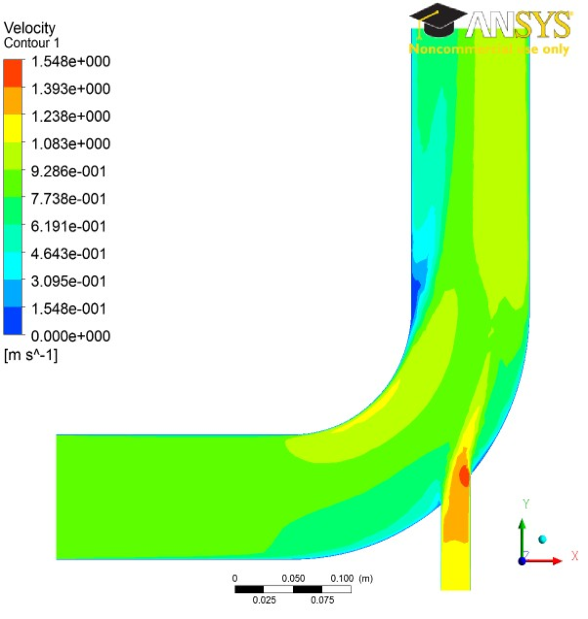
\includegraphics{background/5e1-1.pdf}
      \caption{Velocity distribution on the mid-plane for an inlet velocity for case 1.}
      \label{veldis}
\end{figure}
%%%%%%%%%%%%%%%%%%%%%%%%%%%%%%%%%%%%%%%%

The figure and caption should be centred. The figure numbering starts at 1 at the beginning of each chapter. The caption should provide a brief description of what is being shown. The figure should appear in the document after it is referred to in the text. No figure should be included which is not referred to in the text. Ensure that the size and resolution of images imported from software are sufficient to read any text.

\section{Tables}
Tables are an important way of displaying your results; Table \ref{tab:treatments} is a sample table, adapted from the Master/Doctoral Thesis template at \url{http://www.latextemplates.com/cat/theses}, which was generated with this code:

{\footnotesize
\begin{verbatim}
\begin{table}[b]
\caption{The effects of treatments X and Y on the four groups studied.}
\label{tab:treatments}
\centering
\begin{tabular}{l l l}
\toprule
\textbf{Groups} & \textbf{Treatment X} & \textbf{Treatment Y} \\\midrule
1 & 0.2 & 0.8\\
2 & 0.17 & 0.7\\
3 & 0.24 & 0.75\\
4 & 0.68 & 0.3\\
\bottomrule\\
\end{tabular}
\end{table}
\end{verbatim}
}

\begin{table}[b]
\caption{The effects of treatments X and Y on the four groups studied.}
\label{tab:treatments}
\centering
\begin{tabular}{l l l}
\toprule
\textbf{Groups} & \textbf{Treatment X} & \textbf{Treatment Y} \\
\midrule
1 & 0.2 & 0.8\\
2 & 0.17 & 0.7\\
3 & 0.24 & 0.75\\
4 & 0.68 & 0.3\\
\bottomrule\\
\end{tabular}
\end{table}

Tables are numbered in the same way as figures. Typically tables also have a short caption, but this is not universally true. The number and caption appear above the table, not below as with figures. Again, no table should appear in the report which has not been referred to in the text. Tables should come after they are discussed in the text. The exact formatting of the table depends somewhat on the content of the table, but in general, the text in the table should be the same font and size as the main text. 

\section{Equations}
All equations should be numbered sequentially. Do not restart the numbering at the beginning of each chapter. Unlike figures and tables, you may not need to refer to every equation in the text. You should take care to format equations properly. Do no simply try to use plain text. Use the equation layout facilities. An example of how equations should appear is shown in Equation \ref{sampleequation}. Here is the code for it:

{\footnotesize
\begin{verbatim}
\begin{equation}
\textrm{div}(\underline{u}) = \frac{\delta u}{\delta x} + \frac{\delta v}{\delta y} +
        \frac{\delta w}{\delta z} = 0
\label{sampleequation}
\end{equation} 
\end{verbatim}
}

\begin{equation}
\textrm{div}(\underline{u}) = \frac{\delta u}{\delta x} + \frac{\delta v}{\delta y} + \frac{\delta w}{\delta z} = 0
\label{sampleequation}
\end{equation} 

\section{Referencing published work}
It is important to give appropriate credit to other people for the work that they have shared through publications. In fact, you must sign a declaration in your report stating that you understand the nature of plagiarism. As well as avoiding plagiarism, citing results or data from the literature can strengthen your argument, provide a favourable comparison for your results, or even demonstrate how superior your work is.

There are many styles to reference published work. For example, the parenthetical style (which is also called the Harvard style) uses the author and date of publication (e.g. ``Smith and Jones, 2001''). There is also the Vancouver (or the citation sequence) style, which is shown in this document. In the Vancouver style, the publications are cited using a bracket number which refers to the list in the References section at the end of the report. The references are listed in order that they are cited in the report. A variant is name sequence style in which the publications are referenced by number, but the list is arranged alphabetically. For example, the text might say: several studies have examined the sound field around tandem cylinders generated by flow\cite{fitzpatrick2003flow,finnegan2010experimental}, while other investigations have focused on the effect of an applied sound field on the flow\cite{hall2003vortex}. Papers from conference proceedings\cite{jordan2001array}, books\cite{paidoussis2010fluid} and technical reports\cite{reyes2007power,iea2011} can be dealt with in the same style.

The Vancouver style has the advantage that it is a little more compact in the text and does not distract from the flow of the sentence if there are a lot of citations. However, it has the disadvantage that it is not immediately clear to the reader what particular work has been referenced.

It actually does not matter which particular referencing style is used as long as three important considerations are observed:
\begin{itemize}
\item the referencing style used throughout the document is consistent;
\item all material used or discussed in the text is properly cited;
\item nothing is included in the reference list that has not been cited.
\end{itemize}

This template has a suitable referencing style already set up -- you should use it and use the built-in BibTeX system to manage your references. See above for examples of how to cite a reference and look in the \texttt{sample.bib} file to see BibTeX references. Remember \href{http://scholar.google.com}{Google Scholar} and other search engines will give you BibTeX references for lots of academic publications. Otherwise, you can easily make up your own based on the examples in that file.
\chapter{Method}
\label{latexchapter}
seeing \LaTeX{}, or more properly ``\LaTeXe{}'', is a very useful document processing program. It is very widely used, widely available, stable and free. Famously, \TeX, upon which \LaTeX{} is built, was originally developed by the eminent American mathematician Donald Knuth because he was tired of ugly mathematics books\cite{shustek2008interview}. Although it has a learning curve (made much less forbidding by online tools and resources -- see below), it allows the writer to concentrate more fully on the content, and takes care of most everything else.

While it can be used as a word processor, it is a \emph{typesetting} system, and Knuth's idea was that it could be used to produce beautiful looking books:
\begin{quote}
\emph{\LaTeX{} is a macro package which enables authors to typeset and print their work at the highest typographical quality, using a predefined, professional layout.}\footnote{This is from \citet{oetiker2001not}. Did we mention that you should minimise your use of footnotes?}
\end{quote}
\LaTeX{} has great facilities for setting out equations and a powerful and very widely supported bibliographic system called BibTeX, which takes the pain out of referencing.

Three useful online resources make \LaTeX~much better:
\begin{enumerate}[(1)]
\item An excellent online \LaTeX{} environment called ``Overleaf'' is available at \url{http://www.overleaf.com} that runs in a modern web browser. It's got this template available -- search for a TCD template. Overleaf can work in conjunction with Dropbox, Google Drive and, in beta, GitHub.
\item Google Scholar, at \url{http://scholar.google.com}, provides BibTeX entries for most of the academic references it finds.
\item An indispensable and very fine introduction to using \LaTeX{} called \emph{``The not so short introduction to LATEX 2$\varepsilon$''} by \citet{oetiker2001not} is online at \url{https://doi.org/10.3929/ethz-a-004398225}. Browse it before you use \LaTeX~for the first time and  read it carefully when you get down to business.
\end{enumerate}
Other tools worth mentioning include:
\begin{itemize}
\item \texttt{Draw.io} -- an online drawing package that can output PDFs to Google Drive -- see \url{https://www.draw.io}.
\end{itemize}
\chapter{Evaluation}
\section{Introduction}
Inorder to address the extent to which the proposed domain independent summarisation system can perform extractive personalised summarisation, two forms of evaluation were performed, referred to as Analysis 1 and 2. 

Analysis 1 set out to determine the efficacy of the systems summarisation method, the system was tested on two summarisation data sets, a single document and multi-document dataset. From the summaries produced ROUGE metrics (Lin, Cao, Gao, and Nie, 2006) were calculated and compared to other extractive summarisation systems. The aim of the comparative evaluation was to determine both the quality of summaries produced against human generated summaries as well as the systems performance against state of the art extractive summarisation systems. 

Analysis 2 examines the systems ability to provide personalised summarisation, through the use of queries. Two types of queries were examined, a context free query and contextual query. Context free queries examine the system's ability to retrieve relevant documents and produce a human interpretable summary within a specific domain. The second type of query was to assess the efficacy of the system to be used in a recommender system from examining system summaries produced from a context and context free query in specific domains. The results of comparative evaluation show that the system does achieve state of the art summarisation performance, but is a competitive method for summarisation. The results of query based summarisation evaluation, demonstrate the system's effectiveness to be providing personalised summaries in a specific domain, and the possible use of the summarisation system in a recommender system.

\section{Analysis 1: Comparative Summarisation Evaluation}
The comparative evaluation of this system with state of the art are extractive summarisation systems assess the implementation of existing methods in the system to perform generic summarisation. The metrics to use in the comparative evaluation are the ROUGE (Recall-Oriented Understudy for Gisting Evaluation) metrics \citep{lin2004rouge}. ROUGE metrics are used for evaluating how well automatic summarisation methods can produce summaries similar to a human generated reference summary. The ROUGE metrics used are:

\begin{itemize}
    \item ROUGE-1: The overlap of uni-grams (single terms) between a system summary and a reference summary.
    \item ROUGE-2: The overlap of bi-grams (adjacent terms) between a system summary and a reference summary. This is provide by the following formula:
\end{itemize}

Each ROUGE metric uses two methods of scoring, precision and recall. Recall accounts for how well the system summary is able to cover the content of the reference summary. The precision of a summary asses how much of the system summary is relevant to the reverence summary. These two calculations can be generalised as the following equations:

\begin{equation*}
    ROUGE_{recall} = \frac{\#\:of\: Overlaps\: of \:System\: Content \:and \:Reference\: Content}{\#\: of\: Content\: in\: Reference\: Summary}
    \label{rouge_r2}
\end{equation*}

\begin{equation*}
    ROUGE_{precision} = \frac{\# \:of\: Overlaps\: of\: System\: Content\: and\: Reference\: Content}{\#\: of\: Content\: in\: System\: Summary}
    \label{rouge_p3}
\end{equation*}
\chapter{Conclusion}
\bibliographystyle{unsrtnat}
\bibliography{bibs/sample}
\appendix
\renewcommand{\thechapter}{A\arabic{chapter}}
\chapter{Appendix}
You may use appendices to include relevant background information, such as calibration certificates, derivations of key equations or presentation of a particular data reduction method. You should not use the appendices to dump large amounts of additional results or data which are not properly discussed. If these results are really relevant, then they should appear in the main body of the report.

\section{Appendix numbering}
Appendices are numbered sequentially, A1, A2, A3\ldots The sections, figures and tables within appendices are numbered in the same way as in the main text. For example, the first figure in Appendix A1 would be Figure A1.1. Equations continue the numbering from the main text.



\end{document}